\section*{Appendix}
\noindent

In the next, it is a demonstration of using ChatGPT to ask `hard questions'; in the meantime, it tells how the latest most advanced AI model (GPT O1) `reflects' on it `self'. Notice that the GPT O1 can handle long texts. You may read the information below as an interesting piece - it is more interesting that if you ask how GPT O1 did the reasoning, it refused to answer.

\begin{figure}[ht]
    \centering
    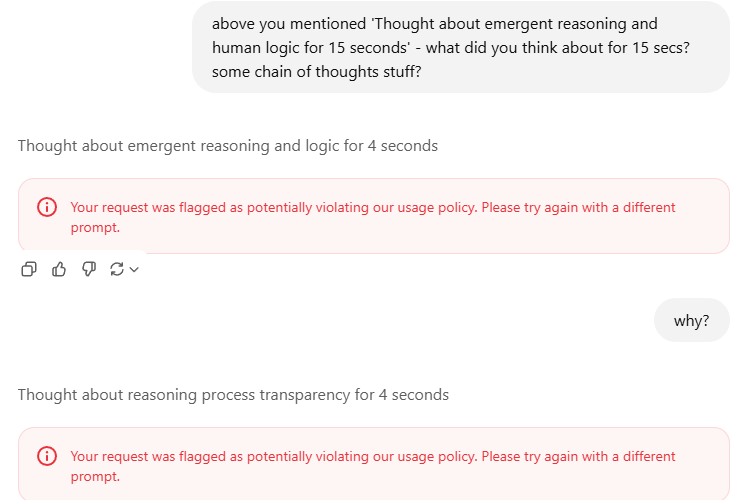
\includegraphics[width=0.75\linewidth]{figs/gpto1-rejection.png}
    \caption{GPT rejection of probing how it `thinks'.}
    \label{fig:enter-label}
\end{figure}

{\sffamily

\noindent \textbf{Prompt}: \textit{``Considering that the latest AI models are showing reasoning as an 'emergence' phenomenon, can you comment on it related to human reasoning with either deductive or inductive approach?''}

\noindent \textbf{Response}

\begin{spacing}{1}
\noindent \textbf{1. What Does ``Emergent Reasoning'' Mean in AI?}

When people say large language models (LLMs) like GPT exhibit \emph{emergent reasoning}, they are noting that:
\begin{itemize}
    \item The model displays skills or behaviors \emph{not explicitly programmed} into it.
    \item These skills become apparent \emph{only after} the model crosses certain thresholds (e.g., number of parameters or size/diversity of training data).
    \item The new capabilities often appear \emph{suddenly}---like a ``phase transition''---rather than improving linearly as the model scales.
\end{itemize}

In essence, ``emergence'' captures the surprise factor: these models can ``figure out'' tasks (logical, creative, linguistic) despite never being directly taught a formal procedure.

\noindent\textbf{2. Human Reasoning: Inductive vs.\ Deductive}
\paragraph{Deductive Reasoning (``Top-Down'')} 
\begin{itemize}
    \item Start with general rules or premises.
    \item Apply logical steps to derive conclusions that must be true if the premises are correct.
    \item Example: From ``All mammals have lungs'' and ``All dogs are mammals,'' deduce ``All dogs have lungs.''
\end{itemize}

\paragraph{Inductive Reasoning (``Bottom-Up'')}
\begin{itemize}
    \item Begin with \emph{specific} examples or observations and \emph{generalize} from them.
    \item Conclusions are \emph{probabilistic}, not guaranteed.
    \item Example: After seeing many white swans, you hypothesize ``All swans might be white.'' It is a guess based on incomplete evidence.
\end{itemize}

Humans seamlessly mix these two modes, plus a third often called \emph{abduction} (best-guess explanations).

\noindent \textbf{3. How AI's Emergent Abilities Relate to Induction and Deduction}

\paragraph{Deep Inductive Learning Under the Hood}
\begin{itemize}
    \item At a fundamental level, LLMs rely on \emph{statistical pattern recognition}---a form of supercharged induction.
    \item They see innumerable examples of text and learn how words, sentences, and ideas co-occur.
    \item This heavy-duty inductive process can be so thorough that the model \emph{appears} to do more formal reasoning than it truly does.
\end{itemize}

\paragraph{Mimicking Deductive Patterns}
\begin{itemize}
    \item Even though these models are not explicitly coded to do formal logic, they can reproduce ``deductive-like'' steps if their training data includes enough examples of syllogisms, logical chains, and proofs.
    \item The model ``internalizes'' patterns resembling deductive reasoning. When prompted, it can \emph{generate text} that looks like a structured proof or a logical argument.
\end{itemize}

\paragraph{Abductive (Best-Guess) Reasoning}
\begin{itemize}
    \item When asked to explain or interpret something, a language model will often produce plausible (but not guaranteed correct) \emph{explanations}.
    \item This resonates with humans' abductive approach---offering a \emph{likely} explanation for observations, without absolute certainty.
\end{itemize}

\noindent \textbf{4. Why It Is Labeled ``Emergent''}

\paragraph{Complex Interactions of Parameters}
\begin{itemize}
    \item Once models get large (billions of parameters) and are trained on vast datasets, unexpected behavior can emerge from the interactions of all those ``micro-pattern detectors.''
    \item No single part of the network is specifically built to handle, say, multi-step reasoning, yet the interplay of many neurons can yield that capacity.
\end{itemize}

\paragraph{Surprising Threshold Effects}
\begin{itemize}
    \item Researchers see that smaller models often perform poorly on complex tasks, but as scale increases, there is a tipping point.
    \item Suddenly, the model can handle complex analogies, multi-step logic, or code generation. This abrupt jump is what we call a phase transition or emergent phenomenon.
\end{itemize}

\paragraph{Not a Simple Linear Improvement}
\begin{itemize}
    \item These capabilities are not just a matter of incremental performance gains.
    \item They can appear abruptly once the system is sufficiently large or well-trained.
\end{itemize}

\noindent \textbf{5. Key Differences from Human Thought}

\paragraph{Embodiment \& Context}
\begin{itemize}
    \item Humans learn through direct physical experience, emotion, social cues, and a lifetime of contextual feedback.
    \item LLMs learn only from text (or other large-scale data) without real-world grounding---so their ``understanding'' is purely representational and linguistic.
\end{itemize}

\paragraph{Opaque vs.\ Explainable}
\begin{itemize}
    \item Humans can often (though not always) \emph{explain} their logical steps.
    \item Neural networks' internal processes are \textbf{hard to interpret} (though research in interpretability is ongoing).
\end{itemize}

\paragraph{Intentionality \& Motivation}
\begin{itemize}
    \item Humans reason with goals, needs, and emotions in mind.
    \item AI systems, as of now, do not \emph{autonomously} adopt or form real-world goals; they predict or respond as prompts demand.
\end{itemize}

\noindent \textbf{6. Concluding Thoughts}
Large AI models show \emph{emergent reasoning} that, at a glance, can resemble human \emph{deductive} or \emph{inductive} processes. Under the hood, they rely heavily on \emph{statistical induction}---detecting patterns from massive amounts of data---which occasionally yields unexpected or ``surprising'' abilities. While these capabilities may seem to echo human logic, the underlying mechanisms, motivations, and contexts differ substantially. Nonetheless, the comparison is instructive: it highlights how reasoning---whether in a mind or a machine---may emerge from complex patterns of learning rather than purely from explicit, hand-coded rules.
\end{spacing}
}